\documentclass[1p]{elsarticle_modified}
%\bibliographystyle{elsarticle-num}

%\usepackage[colorlinks]{hyperref}
%\usepackage{abbrmath_seonhwa} %\Abb, \Ascr, \Acal ,\Abf, \Afrak
\usepackage{amsfonts}
\usepackage{amssymb}
\usepackage{amsmath}
\usepackage{amsthm}
\usepackage{scalefnt}
\usepackage{amsbsy}
\usepackage{kotex}
\usepackage{caption}
\usepackage{subfig}
\usepackage{color}
\usepackage{graphicx}
\usepackage{xcolor} %% white, black, red, green, blue, cyan, magenta, yellow
\usepackage{float}
\usepackage{setspace}
\usepackage{hyperref}

\usepackage{tikz}
\usetikzlibrary{arrows}

\usepackage{multirow}
\usepackage{array} % fixed length table
\usepackage{hhline}

%%%%%%%%%%%%%%%%%%%%%
\makeatletter
\renewcommand*\env@matrix[1][\arraystretch]{%
	\edef\arraystretch{#1}%
	\hskip -\arraycolsep
	\let\@ifnextchar\new@ifnextchar
	\array{*\c@MaxMatrixCols c}}
\makeatother %https://tex.stackexchange.com/questions/14071/how-can-i-increase-the-line-spacing-in-a-matrix
%%%%%%%%%%%%%%%

\usepackage[normalem]{ulem}

\newcommand{\msout}[1]{\ifmmode\text{\sout{\ensuremath{#1}}}\else\sout{#1}\fi}
%SOURCE: \msout is \stkout macro in https://tex.stackexchange.com/questions/20609/strikeout-in-math-mode

\newcommand{\cancel}[1]{
	\ifmmode
	{\color{red}\msout{#1}}
	\else
	{\color{red}\sout{#1}}
	\fi
}

\newcommand{\add}[1]{
	{\color{blue}\uwave{#1}}
}

\newcommand{\replace}[2]{
	\ifmmode
	{\color{red}\msout{#1}}{\color{blue}\uwave{#2}}
	\else
	{\color{red}\sout{#1}}{\color{blue}\uwave{#2}}
	\fi
}

\newcommand{\Sol}{\mathcal{S}} %segment
\newcommand{\D}{D} %diagram
\newcommand{\A}{\mathcal{A}} %arc


%%%%%%%%%%%%%%%%%%%%%%%%%%%%%5 test

\def\sl{\operatorname{\textup{SL}}(2,\Cbb)}
\def\psl{\operatorname{\textup{PSL}}(2,\Cbb)}
\def\quan{\mkern 1mu \triangleright \mkern 1mu}

\theoremstyle{definition}
\newtheorem{thm}{Theorem}[section]
\newtheorem{prop}[thm]{Proposition}
\newtheorem{lem}[thm]{Lemma}
\newtheorem{ques}[thm]{Question}
\newtheorem{cor}[thm]{Corollary}
\newtheorem{defn}[thm]{Definition}
\newtheorem{exam}[thm]{Example}
\newtheorem{rmk}[thm]{Remark}
\newtheorem{alg}[thm]{Algorithm}

\newcommand{\I}{\sqrt{-1}}
\begin{document}

%\begin{frontmatter}
%
%\title{Boundary parabolic representations of knots up to 8 crossings}
%
%%% Group authors per affiliation:
%\author{Yunhi Cho} 
%\address{Department of Mathematics, University of Seoul, Seoul, Korea}
%\ead{yhcho@uos.ac.kr}
%
%
%\author{Seonhwa Kim} %\fnref{s_kim}}
%\address{Center for Geometry and Physics, Institute for Basic Science, Pohang, 37673, Korea}
%\ead{ryeona17@ibs.re.kr}
%
%\author{Hyuk Kim}
%\address{Department of Mathematical Sciences, Seoul National University, Seoul 08826, Korea}
%\ead{hyukkim@snu.ac.kr}
%
%\author{Seokbeom Yoon}
%\address{Department of Mathematical Sciences, Seoul National University, Seoul, 08826,  Korea}
%\ead{sbyoon15@snu.ac.kr}
%
%\begin{abstract}
%We find all boundary parabolic representation of knots up to 8 crossings.
%
%\end{abstract}
%\begin{keyword}
%    \MSC[2010] 57M25 
%\end{keyword}
%
%\end{frontmatter}

%\linenumbers
%\tableofcontents
%
\newcommand\colored[1]{\textcolor{white}{\rule[-0.35ex]{0.8em}{1.4ex}}\kern-0.8em\color{red} #1}%
%\newcommand\colored[1]{\textcolor{white}{ #1}\kern-2.17ex	\textcolor{white}{ #1}\kern-1.81ex	\textcolor{white}{ #1}\kern-2.15ex\color{red}#1	}

{\Large $\underline{12a_{0003}~(K12a_{0003})}$}

\setlength{\tabcolsep}{10pt}
\renewcommand{\arraystretch}{1.6}
\vspace{1cm}\begin{tabular}{m{100pt}>{\centering\arraybackslash}m{274pt}}
\multirow{5}{120pt}{
	\centering
	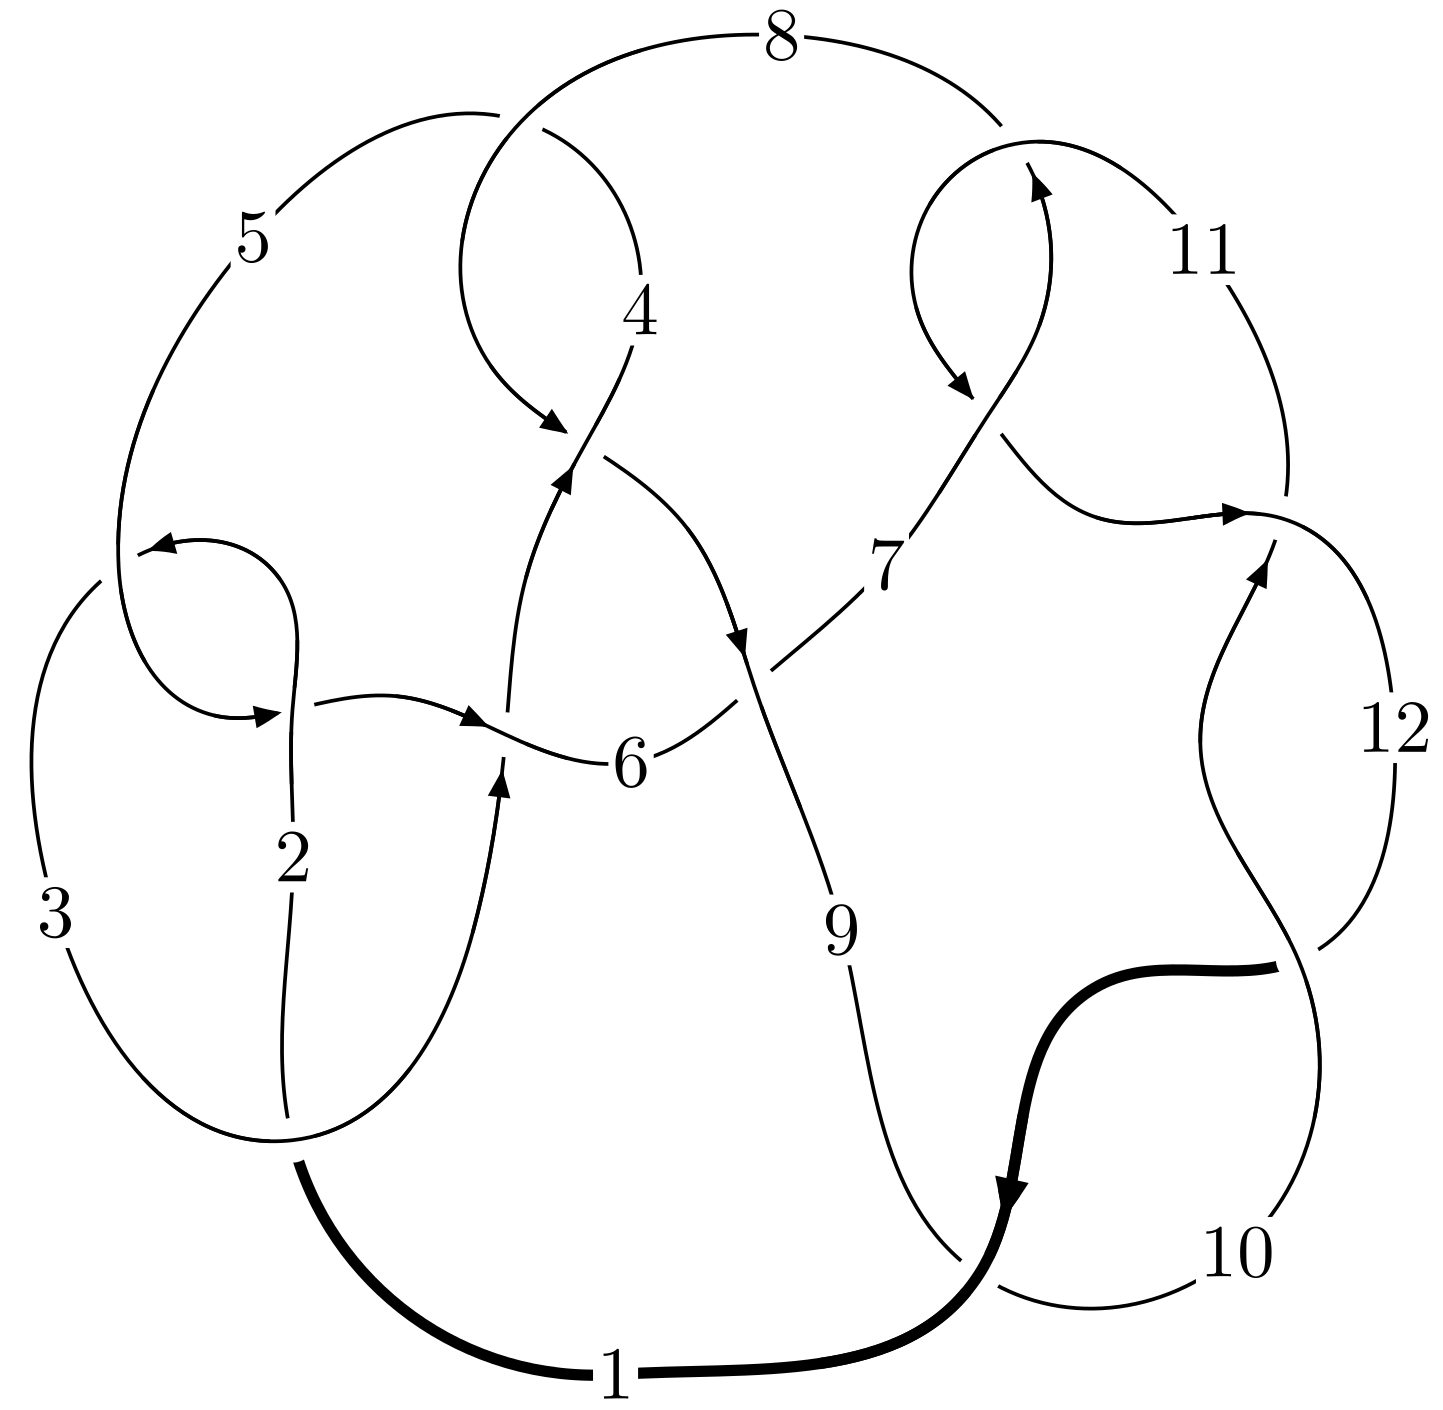
\includegraphics[width=112pt]{../../../GIT/diagram.site/Diagrams/png/804_12a_0003.png}\\
\ \ \ A knot diagram\footnotemark}&
\allowdisplaybreaks
\textbf{Linearized knot diagam} \\
\cline{2-2}
 &
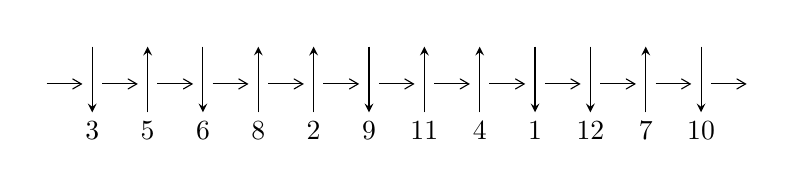
\begin{tikzpicture}[x=20pt, y=17pt]
	% nodes
	\node (C0) at (0, 0) {};
	\node (C1) at (1, 0) {};
	\node (C1U) at (1, +1) {};
	\node (C1D) at (1, -1) {3};

	\node (C2) at (2, 0) {};
	\node (C2U) at (2, +1) {};
	\node (C2D) at (2, -1) {5};

	\node (C3) at (3, 0) {};
	\node (C3U) at (3, +1) {};
	\node (C3D) at (3, -1) {6};

	\node (C4) at (4, 0) {};
	\node (C4U) at (4, +1) {};
	\node (C4D) at (4, -1) {8};

	\node (C5) at (5, 0) {};
	\node (C5U) at (5, +1) {};
	\node (C5D) at (5, -1) {2};

	\node (C6) at (6, 0) {};
	\node (C6U) at (6, +1) {};
	\node (C6D) at (6, -1) {9};

	\node (C7) at (7, 0) {};
	\node (C7U) at (7, +1) {};
	\node (C7D) at (7, -1) {11};

	\node (C8) at (8, 0) {};
	\node (C8U) at (8, +1) {};
	\node (C8D) at (8, -1) {4};

	\node (C9) at (9, 0) {};
	\node (C9U) at (9, +1) {};
	\node (C9D) at (9, -1) {1};

	\node (C10) at (10, 0) {};
	\node (C10U) at (10, +1) {};
	\node (C10D) at (10, -1) {12};

	\node (C11) at (11, 0) {};
	\node (C11U) at (11, +1) {};
	\node (C11D) at (11, -1) {7};

	\node (C12) at (12, 0) {};
	\node (C12U) at (12, +1) {};
	\node (C12D) at (12, -1) {10};
	\node (C13) at (13, 0) {};

	% arrows
	\draw[->,>={angle 60}]
	(C0) edge (C1) (C1) edge (C2) (C2) edge (C3) (C3) edge (C4) (C4) edge (C5) (C5) edge (C6) (C6) edge (C7) (C7) edge (C8) (C8) edge (C9) (C9) edge (C10) (C10) edge (C11) (C11) edge (C12) (C12) edge (C13) ;	\draw[->,>=stealth]
	(C1U) edge (C1D) (C2D) edge (C2U) (C3U) edge (C3D) (C4D) edge (C4U) (C5D) edge (C5U) (C6U) edge (C6D) (C7D) edge (C7U) (C8D) edge (C8U) (C9U) edge (C9D) (C10U) edge (C10D) (C11D) edge (C11U) (C12U) edge (C12D) ;
	\end{tikzpicture} \\
\hhline{~~} \\& 
\textbf{Solving Sequence} \\ \cline{2-2} 
 &
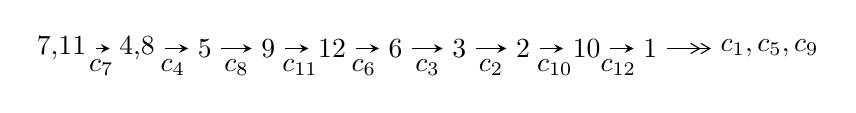
\begin{tikzpicture}[x=23pt, y=7pt]
	% node
	\node (A0) at (-1/8, 0) {7,11};
	\node (A1) at (17/16, 0) {4,8};
	\node (A2) at (17/8, 0) {5};
	\node (A3) at (25/8, 0) {9};
	\node (A4) at (33/8, 0) {12};
	\node (A5) at (41/8, 0) {6};
	\node (A6) at (49/8, 0) {3};
	\node (A7) at (57/8, 0) {2};
	\node (A8) at (65/8, 0) {10};
	\node (A9) at (73/8, 0) {1};
	\node (C1) at (1/2, -1) {$c_{7}$};
	\node (C2) at (13/8, -1) {$c_{4}$};
	\node (C3) at (21/8, -1) {$c_{8}$};
	\node (C4) at (29/8, -1) {$c_{11}$};
	\node (C5) at (37/8, -1) {$c_{6}$};
	\node (C6) at (45/8, -1) {$c_{3}$};
	\node (C7) at (53/8, -1) {$c_{2}$};
	\node (C8) at (61/8, -1) {$c_{10}$};
	\node (C9) at (69/8, -1) {$c_{12}$};
	\node (A10) at (11, 0) {$c_{1},c_{5},c_{9}$};

	% edge
	\draw[->,>=stealth]	
	(A0) edge (A1) (A1) edge (A2) (A2) edge (A3) (A3) edge (A4) (A4) edge (A5) (A5) edge (A6) (A6) edge (A7) (A7) edge (A8) (A8) edge (A9) ;
	\draw[->>,>={angle 60}]	
	(A9) edge (A10);
\end{tikzpicture} \\ 

\end{tabular} \\

\footnotetext{
The image of knot diagram is generated by the software ``\textbf{Draw programme}" developed by Andrew Bartholomew(\url{http://www.layer8.co.uk/maths/draw/index.htm\#Running-draw}), where we modified some parts for our purpose(\url{https://github.com/CATsTAILs/LinksPainter}).
}\phantom \\ \newline 
\centering \textbf{Ideals for irreducible components\footnotemark of $X_{\text{par}}$} 
 
\begin{align*}
I^u_{1}&=\langle 
-8 u^{91}-7 u^{90}+\cdots+2 b-8 u,\;-8 u^{91}-24 u^{90}+\cdots+2 a-9,\;u^{92}+3 u^{91}+\cdots+3 u^2+1\rangle \\
I^u_{2}&=\langle 
u^2 a+b,\;u^2 a- u^3+a^2- a u+2 u^2+a-2 u,\;u^4- u^3+u^2+1\rangle \\
\\
\end{align*}
\raggedright * 2 irreducible components of $\dim_{\mathbb{C}}=0$, with total 100 representations.\\
\footnotetext{All coefficients of polynomials are rational numbers. But the coefficients are sometimes approximated in decimal forms when there is not enough margin.}
\newpage
\renewcommand{\arraystretch}{1}
\centering \section*{I. $I^u_{1}= \langle -8 u^{91}-7 u^{90}+\cdots+2 b-8 u,\;-8 u^{91}-24 u^{90}+\cdots+2 a-9,\;u^{92}+3 u^{91}+\cdots+3 u^2+1 \rangle$}
\flushleft \textbf{(i) Arc colorings}\\
\begin{tabular}{m{7pt} m{180pt} m{7pt} m{180pt} }
\flushright $a_{7}=$&$\begin{pmatrix}1\\0\end{pmatrix}$ \\
\flushright $a_{11}=$&$\begin{pmatrix}0\\u\end{pmatrix}$ \\
\flushright $a_{4}=$&$\begin{pmatrix}4 u^{91}+12 u^{90}+\cdots+13 u^2+\frac{9}{2}\\4 u^{91}+\frac{7}{2} u^{90}+\cdots-\frac{9}{2} u^2+4 u\end{pmatrix}$ \\
\flushright $a_{8}=$&$\begin{pmatrix}1\\- u^2\end{pmatrix}$ \\
\flushright $a_{5}=$&$\begin{pmatrix}4 u^{91}+12 u^{90}+\cdots+13 u^2+\frac{9}{2}\\4 u^{91}+\frac{9}{2} u^{90}+\cdots-\frac{9}{2} u^2+4 u\end{pmatrix}$ \\
\flushright $a_{9}=$&$\begin{pmatrix}u^7+2 u^3\\u^7+u^5+2 u^3+u\end{pmatrix}$ \\
\flushright $a_{12}=$&$\begin{pmatrix}u\\u\end{pmatrix}$ \\
\flushright $a_{6}=$&$\begin{pmatrix}- u^{14}- u^{12}-4 u^{10}-3 u^8-4 u^6-2 u^4+1\\- u^{14}-2 u^{12}-5 u^{10}-6 u^8-6 u^6-4 u^4- u^2\end{pmatrix}$ \\
\flushright $a_{3}=$&$\begin{pmatrix}\frac{3}{2} u^{91}+6 u^{90}+\cdots+u+3\\\frac{3}{2} u^{91}+u^{90}+\cdots-3 u^2+\frac{5}{2} u\end{pmatrix}$ \\
\flushright $a_{2}=$&$\begin{pmatrix}-\frac{1}{2} u^{91}- u^{90}+\cdots-\frac{13}{2} u^3-2 u^2\\-\frac{1}{2} u^{91}-5 u^{89}+\cdots-\frac{3}{2} u^3-\frac{1}{2} u\end{pmatrix}$ \\
\flushright $a_{10}=$&$\begin{pmatrix}u^3\\u^3+u\end{pmatrix}$ \\
\flushright $a_{1}=$&$\begin{pmatrix}u^5+u\\u^5+u^3+u\end{pmatrix}$\\&\end{tabular}
\flushleft \textbf{(ii) Obstruction class $= -1$}\\~\\
\flushleft \textbf{(iii) Cusp Shapes $= \frac{9}{2} u^{91}+7 u^{90}+\cdots+14 u-\frac{1}{2}$}\\~\\
\newpage\renewcommand{\arraystretch}{1}
\flushleft \textbf{(iv) u-Polynomials at the component}\newline \\
\begin{tabular}{m{50pt}|m{274pt}}
Crossings & \hspace{64pt}u-Polynomials at each crossing \\
\hline $$\begin{aligned}c_{1}\end{aligned}$$&$\begin{aligned}
&u^{92}+45 u^{91}+\cdots+6 u+1
\end{aligned}$\\
\hline $$\begin{aligned}c_{2},c_{5}\end{aligned}$$&$\begin{aligned}
&u^{92}+5 u^{91}+\cdots+6 u+1
\end{aligned}$\\
\hline $$\begin{aligned}c_{3}\end{aligned}$$&$\begin{aligned}
&u^{92}-5 u^{91}+\cdots-57066 u+15489
\end{aligned}$\\
\hline $$\begin{aligned}c_{4},c_{8}\end{aligned}$$&$\begin{aligned}
&u^{92}- u^{91}+\cdots+896 u+256
\end{aligned}$\\
\hline $$\begin{aligned}c_{6}\end{aligned}$$&$\begin{aligned}
&u^{92}-3 u^{91}+\cdots-10300 u+2425
\end{aligned}$\\
\hline $$\begin{aligned}c_{7},c_{11}\end{aligned}$$&$\begin{aligned}
&u^{92}-3 u^{91}+\cdots+3 u^2+1
\end{aligned}$\\
\hline $$\begin{aligned}c_{9},c_{10},c_{12}\end{aligned}$$&$\begin{aligned}
&u^{92}+23 u^{91}+\cdots+6 u+1
\end{aligned}$\\
\hline
\end{tabular}\\~\\
\newpage\renewcommand{\arraystretch}{1}
\flushleft \textbf{(v) Riley Polynomials at the component}\newline \\
\begin{tabular}{m{50pt}|m{274pt}}
Crossings & \hspace{64pt}Riley Polynomials at each crossing \\
\hline $$\begin{aligned}c_{1}\end{aligned}$$&$\begin{aligned}
&y^{92}+9 y^{91}+\cdots+46 y+1
\end{aligned}$\\
\hline $$\begin{aligned}c_{2},c_{5}\end{aligned}$$&$\begin{aligned}
&y^{92}+45 y^{91}+\cdots+6 y+1
\end{aligned}$\\
\hline $$\begin{aligned}c_{3}\end{aligned}$$&$\begin{aligned}
&y^{92}-27 y^{91}+\cdots-1648615266 y+239909121
\end{aligned}$\\
\hline $$\begin{aligned}c_{4},c_{8}\end{aligned}$$&$\begin{aligned}
&y^{92}+45 y^{91}+\cdots+1327104 y+65536
\end{aligned}$\\
\hline $$\begin{aligned}c_{6}\end{aligned}$$&$\begin{aligned}
&y^{92}-5 y^{91}+\cdots-386124150 y+5880625
\end{aligned}$\\
\hline $$\begin{aligned}c_{7},c_{11}\end{aligned}$$&$\begin{aligned}
&y^{92}+23 y^{91}+\cdots+6 y+1
\end{aligned}$\\
\hline $$\begin{aligned}c_{9},c_{10},c_{12}\end{aligned}$$&$\begin{aligned}
&y^{92}+95 y^{91}+\cdots+46 y+1
\end{aligned}$\\
\hline
\end{tabular}\\~\\
\newpage\flushleft \textbf{(vi) Complex Volumes and Cusp Shapes}
$$\begin{array}{c|c|c}  
\text{Solutions to }I^u_{1}& \I (\text{vol} + \sqrt{-1}CS) & \text{Cusp shape}\\
 \hline 
\begin{aligned}
u &= -0.693479 + 0.720110 I \\
a &= \phantom{-}0.620794 + 0.272394 I \\
b &= -0.270197 - 0.526769 I\end{aligned}
 & -2.50471 + 1.32727 I & \phantom{-0.000000 } 0 \\ \hline\begin{aligned}
u &= -0.693479 - 0.720110 I \\
a &= \phantom{-}0.620794 - 0.272394 I \\
b &= -0.270197 + 0.526769 I\end{aligned}
 & -2.50471 - 1.32727 I & \phantom{-0.000000 } 0 \\ \hline\begin{aligned}
u &= \phantom{-}0.137759 + 0.991033 I \\
a &= \phantom{-}0.96131 - 2.44396 I \\
b &= -0.226283 - 1.348390 I\end{aligned}
 & -7.08384 - 6.20405 I & \phantom{-0.000000 } 0 \\ \hline\begin{aligned}
u &= \phantom{-}0.137759 - 0.991033 I \\
a &= \phantom{-}0.96131 + 2.44396 I \\
b &= -0.226283 + 1.348390 I\end{aligned}
 & -7.08384 + 6.20405 I & \phantom{-0.000000 } 0 \\ \hline\begin{aligned}
u &= \phantom{-}0.198705 + 0.989118 I \\
a &= \phantom{-}1.00312 - 2.59715 I \\
b &= -0.30023 - 1.51641 I\end{aligned}
 & -8.51146 + 2.14258 I & \phantom{-0.000000 } 0 \\ \hline\begin{aligned}
u &= \phantom{-}0.198705 - 0.989118 I \\
a &= \phantom{-}1.00312 + 2.59715 I \\
b &= -0.30023 + 1.51641 I\end{aligned}
 & -8.51146 - 2.14258 I & \phantom{-0.000000 } 0 \\ \hline\begin{aligned}
u &= -0.323111 + 0.935504 I \\
a &= \phantom{-}1.045650 - 0.704782 I \\
b &= \phantom{-}0.190797 - 0.218407 I\end{aligned}
 & -2.70385 - 6.14257 I & \phantom{-0.000000 } 0 \\ \hline\begin{aligned}
u &= -0.323111 - 0.935504 I \\
a &= \phantom{-}1.045650 + 0.704782 I \\
b &= \phantom{-}0.190797 + 0.218407 I\end{aligned}
 & -2.70385 + 6.14257 I & \phantom{-0.000000 } 0 \\ \hline\begin{aligned}
u &= \phantom{-}0.156856 + 0.960463 I \\
a &= -0.88681 + 2.52095 I \\
b &= \phantom{-}0.338463 + 1.363710 I\end{aligned}
 & -4.30279 - 1.37565 I & \phantom{-0.000000 } 0 \\ \hline\begin{aligned}
u &= \phantom{-}0.156856 - 0.960463 I \\
a &= -0.88681 - 2.52095 I \\
b &= \phantom{-}0.338463 - 1.363710 I\end{aligned}
 & -4.30279 + 1.37565 I & \phantom{-0.000000 } 0\\
 \hline 
 \end{array}$$\newpage$$\begin{array}{c|c|c}  
\text{Solutions to }I^u_{1}& \I (\text{vol} + \sqrt{-1}CS) & \text{Cusp shape}\\
 \hline 
\begin{aligned}
u &= \phantom{-}0.362369 + 0.977795 I \\
a &= \phantom{-}1.23952 - 2.65966 I \\
b &= -0.32670 - 1.89189 I\end{aligned}
 & -3.12348 + 7.02740 I & \phantom{-0.000000 } 0 \\ \hline\begin{aligned}
u &= \phantom{-}0.362369 - 0.977795 I \\
a &= \phantom{-}1.23952 + 2.65966 I \\
b &= -0.32670 + 1.89189 I\end{aligned}
 & -3.12348 - 7.02740 I & \phantom{-0.000000 } 0 \\ \hline\begin{aligned}
u &= \phantom{-}0.331238 + 0.895820 I \\
a &= \phantom{-}1.32460 - 2.96062 I \\
b &= -0.54342 - 1.96702 I\end{aligned}
 & -0.69918 + 4.80724 I & \phantom{-0.000000 } 0 \\ \hline\begin{aligned}
u &= \phantom{-}0.331238 - 0.895820 I \\
a &= \phantom{-}1.32460 + 2.96062 I \\
b &= -0.54342 + 1.96702 I\end{aligned}
 & -0.69918 - 4.80724 I & \phantom{-0.000000 } 0 \\ \hline\begin{aligned}
u &= \phantom{-}0.327350 + 0.992443 I \\
a &= -1.17765 + 2.68899 I \\
b &= \phantom{-}0.32569 + 1.83006 I\end{aligned}
 & -7.76770 + 3.77242 I & \phantom{-0.000000 } 0 \\ \hline\begin{aligned}
u &= \phantom{-}0.327350 - 0.992443 I \\
a &= -1.17765 - 2.68899 I \\
b &= \phantom{-}0.32569 - 1.83006 I\end{aligned}
 & -7.76770 - 3.77242 I & \phantom{-0.000000 } 0 \\ \hline\begin{aligned}
u &= -0.233602 + 0.910910 I \\
a &= \phantom{-}0.846140 - 1.033200 I \\
b &= \phantom{-}0.094081 - 0.372222 I\end{aligned}
 & -3.23122 + 1.00291 I & \phantom{-0.000000 } 0 \\ \hline\begin{aligned}
u &= -0.233602 - 0.910910 I \\
a &= \phantom{-}0.846140 + 1.033200 I \\
b &= \phantom{-}0.094081 + 0.372222 I\end{aligned}
 & -3.23122 - 1.00291 I & \phantom{-0.000000 } 0 \\ \hline\begin{aligned}
u &= \phantom{-}0.372819 + 0.996928 I \\
a &= -1.21269 + 2.62443 I \\
b &= \phantom{-}0.29853 + 1.89032 I\end{aligned}
 & -5.72377 + 12.12640 I & \phantom{-0.000000 } 0 \\ \hline\begin{aligned}
u &= \phantom{-}0.372819 - 0.996928 I \\
a &= -1.21269 - 2.62443 I \\
b &= \phantom{-}0.29853 - 1.89032 I\end{aligned}
 & -5.72377 - 12.12640 I & \phantom{-0.000000 } 0\\
 \hline 
 \end{array}$$\newpage$$\begin{array}{c|c|c}  
\text{Solutions to }I^u_{1}& \I (\text{vol} + \sqrt{-1}CS) & \text{Cusp shape}\\
 \hline 
\begin{aligned}
u &= -0.335045 + 0.866771 I \\
a &= -0.790918 + 0.569269 I \\
b &= -0.082338 + 0.179534 I\end{aligned}
 & -0.38070 - 2.07048 I & \phantom{-0.000000 } 0 \\ \hline\begin{aligned}
u &= -0.335045 - 0.866771 I \\
a &= -0.790918 - 0.569269 I \\
b &= -0.082338 - 0.179534 I\end{aligned}
 & -0.38070 + 2.07048 I & \phantom{-0.000000 } 0 \\ \hline\begin{aligned}
u &= \phantom{-}0.284068 + 0.860333 I \\
a &= -1.02927 + 3.20717 I \\
b &= \phantom{-}0.80719 + 1.83021 I\end{aligned}
 & -1.058000 - 0.279101 I & -6.91300 + 0. I\phantom{ +0.000000I} \\ \hline\begin{aligned}
u &= \phantom{-}0.284068 - 0.860333 I \\
a &= -1.02927 - 3.20717 I \\
b &= \phantom{-}0.80719 - 1.83021 I\end{aligned}
 & -1.058000 + 0.279101 I & -6.91300 + 0. I\phantom{ +0.000000I} \\ \hline\begin{aligned}
u &= -0.427081 + 0.798857 I \\
a &= -0.713657 + 0.121097 I \\
b &= -0.0301309 + 0.0996555 I\end{aligned}
 & -0.06045 - 1.88314 I & \phantom{-0.000000 } 0 \\ \hline\begin{aligned}
u &= -0.427081 - 0.798857 I \\
a &= -0.713657 - 0.121097 I \\
b &= -0.0301309 - 0.0996555 I\end{aligned}
 & -0.06045 + 1.88314 I & \phantom{-0.000000 } 0 \\ \hline\begin{aligned}
u &= -0.653453 + 0.885413 I \\
a &= \phantom{-}1.046580 + 0.507386 I \\
b &= -0.445709 + 0.180341 I\end{aligned}
 & -2.57991 + 1.44003 I & \phantom{-0.000000 } 0 \\ \hline\begin{aligned}
u &= -0.653453 - 0.885413 I \\
a &= \phantom{-}1.046580 - 0.507386 I \\
b &= -0.445709 - 0.180341 I\end{aligned}
 & -2.57991 - 1.44003 I & \phantom{-0.000000 } 0 \\ \hline\begin{aligned}
u &= -0.668456 + 0.553251 I \\
a &= \phantom{-}0.751735 + 0.111879 I \\
b &= \phantom{-}0.203275 - 0.551941 I\end{aligned}
 & -1.70083 - 6.18476 I & \phantom{-0.000000 -}0. + 7.03177 I \\ \hline\begin{aligned}
u &= -0.668456 - 0.553251 I \\
a &= \phantom{-}0.751735 - 0.111879 I \\
b &= \phantom{-}0.203275 + 0.551941 I\end{aligned}
 & -1.70083 + 6.18476 I & \phantom{-0.000000 } 0. - 7.03177 I\\
 \hline 
 \end{array}$$\newpage$$\begin{array}{c|c|c}  
\text{Solutions to }I^u_{1}& \I (\text{vol} + \sqrt{-1}CS) & \text{Cusp shape}\\
 \hline 
\begin{aligned}
u &= -0.735212 + 0.893849 I \\
a &= -0.937046 - 0.931574 I \\
b &= \phantom{-}1.053810 - 0.287790 I\end{aligned}
 & \phantom{-}0.60676 - 2.79602 I & \phantom{-0.000000 } 0 \\ \hline\begin{aligned}
u &= -0.735212 - 0.893849 I \\
a &= -0.937046 + 0.931574 I \\
b &= \phantom{-}1.053810 + 0.287790 I\end{aligned}
 & \phantom{-}0.60676 + 2.79602 I & \phantom{-0.000000 } 0 \\ \hline\begin{aligned}
u &= \phantom{-}0.812449 + 0.852311 I \\
a &= \phantom{-}0.778077 - 0.513337 I \\
b &= \phantom{-}0.344350 - 0.859731 I\end{aligned}
 & \phantom{-}3.10988 + 3.40561 I & \phantom{-0.000000 } 0 \\ \hline\begin{aligned}
u &= \phantom{-}0.812449 - 0.852311 I \\
a &= \phantom{-}0.778077 + 0.513337 I \\
b &= \phantom{-}0.344350 + 0.859731 I\end{aligned}
 & \phantom{-}3.10988 - 3.40561 I & \phantom{-0.000000 } 0 \\ \hline\begin{aligned}
u &= -0.863378 + 0.806506 I \\
a &= \phantom{-}0.305173 - 0.349815 I \\
b &= \phantom{-}0.99000 + 1.67872 I\end{aligned}
 & -0.06562 + 2.04123 I & \phantom{-0.000000 } 0 \\ \hline\begin{aligned}
u &= -0.863378 - 0.806506 I \\
a &= \phantom{-}0.305173 + 0.349815 I \\
b &= \phantom{-}0.99000 - 1.67872 I\end{aligned}
 & -0.06562 - 2.04123 I & \phantom{-0.000000 } 0 \\ \hline\begin{aligned}
u &= -0.727666 + 0.941058 I \\
a &= \phantom{-}1.26854 + 0.94209 I \\
b &= -0.832530 + 0.747199 I\end{aligned}
 & -3.02486 - 6.79677 I & \phantom{-0.000000 } 0 \\ \hline\begin{aligned}
u &= -0.727666 - 0.941058 I \\
a &= \phantom{-}1.26854 - 0.94209 I \\
b &= -0.832530 - 0.747199 I\end{aligned}
 & -3.02486 + 6.79677 I & \phantom{-0.000000 } 0 \\ \hline\begin{aligned}
u &= \phantom{-}0.854175 + 0.832632 I \\
a &= \phantom{-}0.906340 - 0.293878 I \\
b &= \phantom{-}0.603181 - 0.774979 I\end{aligned}
 & \phantom{-}4.74497 - 3.82999 I & \phantom{-0.000000 } 0 \\ \hline\begin{aligned}
u &= \phantom{-}0.854175 - 0.832632 I \\
a &= \phantom{-}0.906340 + 0.293878 I \\
b &= \phantom{-}0.603181 + 0.774979 I\end{aligned}
 & \phantom{-}4.74497 + 3.82999 I & \phantom{-0.000000 } 0\\
 \hline 
 \end{array}$$\newpage$$\begin{array}{c|c|c}  
\text{Solutions to }I^u_{1}& \I (\text{vol} + \sqrt{-1}CS) & \text{Cusp shape}\\
 \hline 
\begin{aligned}
u &= -0.841430 + 0.856318 I \\
a &= \phantom{-}0.476794 - 1.094360 I \\
b &= \phantom{-}1.98535 + 1.56704 I\end{aligned}
 & \phantom{-}5.88107 - 3.20332 I & \phantom{-0.000000 } 0 \\ \hline\begin{aligned}
u &= -0.841430 - 0.856318 I \\
a &= \phantom{-}0.476794 + 1.094360 I \\
b &= \phantom{-}1.98535 - 1.56704 I\end{aligned}
 & \phantom{-}5.88107 + 3.20332 I & \phantom{-0.000000 } 0 \\ \hline\begin{aligned}
u &= -0.854533 + 0.845597 I \\
a &= -0.579807 + 0.786808 I \\
b &= -1.63230 - 1.81549 I\end{aligned}
 & \phantom{-}6.71455 + 2.11791 I & \phantom{-0.000000 } 0 \\ \hline\begin{aligned}
u &= -0.854533 - 0.845597 I \\
a &= -0.579807 - 0.786808 I \\
b &= -1.63230 + 1.81549 I\end{aligned}
 & \phantom{-}6.71455 - 2.11791 I & \phantom{-0.000000 } 0 \\ \hline\begin{aligned}
u &= -0.878203 + 0.822809 I \\
a &= -0.539802 + 0.321431 I \\
b &= -1.06748 - 1.95673 I\end{aligned}
 & \phantom{-}4.90178 + 4.97100 I & \phantom{-0.000000 } 0 \\ \hline\begin{aligned}
u &= -0.878203 - 0.822809 I \\
a &= -0.539802 - 0.321431 I \\
b &= -1.06748 + 1.95673 I\end{aligned}
 & \phantom{-}4.90178 - 4.97100 I & \phantom{-0.000000 } 0 \\ \hline\begin{aligned}
u &= \phantom{-}0.852963 + 0.852144 I \\
a &= -0.800671 + 0.266145 I \\
b &= -0.530329 + 0.676515 I\end{aligned}
 & \phantom{-}6.97495 + 0.83818 I & \phantom{-0.000000 } 0 \\ \hline\begin{aligned}
u &= \phantom{-}0.852963 - 0.852144 I \\
a &= -0.800671 - 0.266145 I \\
b &= -0.530329 - 0.676515 I\end{aligned}
 & \phantom{-}6.97495 - 0.83818 I & \phantom{-0.000000 } 0 \\ \hline\begin{aligned}
u &= -0.887379 + 0.818068 I \\
a &= \phantom{-}0.538898 - 0.204942 I \\
b &= \phantom{-}0.93986 + 2.00633 I\end{aligned}
 & \phantom{-}2.49798 + 10.21280 I & \phantom{-0.000000 } 0 \\ \hline\begin{aligned}
u &= -0.887379 - 0.818068 I \\
a &= \phantom{-}0.538898 + 0.204942 I \\
b &= \phantom{-}0.93986 - 2.00633 I\end{aligned}
 & \phantom{-}2.49798 - 10.21280 I & \phantom{-0.000000 } 0\\
 \hline 
 \end{array}$$\newpage$$\begin{array}{c|c|c}  
\text{Solutions to }I^u_{1}& \I (\text{vol} + \sqrt{-1}CS) & \text{Cusp shape}\\
 \hline 
\begin{aligned}
u &= -0.562885 + 0.546500 I \\
a &= -0.780726 - 0.216705 I \\
b &= -0.215186 + 0.354968 I\end{aligned}
 & \phantom{-}0.65863 - 1.83346 I & \phantom{-}3.56478 + 4.16412 I \\ \hline\begin{aligned}
u &= -0.562885 - 0.546500 I \\
a &= -0.780726 + 0.216705 I \\
b &= -0.215186 - 0.354968 I\end{aligned}
 & \phantom{-}0.65863 + 1.83346 I & \phantom{-}3.56478 - 4.16412 I \\ \hline\begin{aligned}
u &= \phantom{-}0.791164 + 0.932385 I \\
a &= -0.309000 + 0.907116 I \\
b &= \phantom{-}0.212321 + 0.879598 I\end{aligned}
 & \phantom{-}2.86189 + 2.60803 I & \phantom{-0.000000 } 0 \\ \hline\begin{aligned}
u &= \phantom{-}0.791164 - 0.932385 I \\
a &= -0.309000 - 0.907116 I \\
b &= \phantom{-}0.212321 - 0.879598 I\end{aligned}
 & \phantom{-}2.86189 - 2.60803 I & \phantom{-0.000000 } 0 \\ \hline\begin{aligned}
u &= \phantom{-}0.868970 + 0.886551 I \\
a &= -0.621192 + 0.030063 I \\
b &= -0.516416 + 0.357413 I\end{aligned}
 & \phantom{-}7.82228 + 2.10226 I & \phantom{-0.000000 } 0 \\ \hline\begin{aligned}
u &= \phantom{-}0.868970 - 0.886551 I \\
a &= -0.621192 - 0.030063 I \\
b &= -0.516416 - 0.357413 I\end{aligned}
 & \phantom{-}7.82228 - 2.10226 I & \phantom{-0.000000 } 0 \\ \hline\begin{aligned}
u &= -0.811671 + 0.940994 I \\
a &= -1.53622 - 1.73359 I \\
b &= \phantom{-}1.94836 - 1.80046 I\end{aligned}
 & \phantom{-}5.61602 - 2.96104 I & \phantom{-0.000000 } 0 \\ \hline\begin{aligned}
u &= -0.811671 - 0.940994 I \\
a &= -1.53622 + 1.73359 I \\
b &= \phantom{-}1.94836 + 1.80046 I\end{aligned}
 & \phantom{-}5.61602 + 2.96104 I & \phantom{-0.000000 } 0 \\ \hline\begin{aligned}
u &= -0.101784 + 0.749735 I \\
a &= -0.06658 + 1.44004 I \\
b &= \phantom{-}0.335460 + 0.379358 I\end{aligned}
 & -1.52871 - 1.62635 I & -6.71018 + 4.39612 I \\ \hline\begin{aligned}
u &= -0.101784 - 0.749735 I \\
a &= -0.06658 - 1.44004 I \\
b &= \phantom{-}0.335460 - 0.379358 I\end{aligned}
 & -1.52871 + 1.62635 I & -6.71018 - 4.39612 I\\
 \hline 
 \end{array}$$\newpage$$\begin{array}{c|c|c}  
\text{Solutions to }I^u_{1}& \I (\text{vol} + \sqrt{-1}CS) & \text{Cusp shape}\\
 \hline 
\begin{aligned}
u &= \phantom{-}0.817197 + 0.949188 I \\
a &= \phantom{-}0.048839 - 0.862965 I \\
b &= -0.386052 - 0.727595 I\end{aligned}
 & \phantom{-}6.67073 + 5.37797 I & \phantom{-0.000000 } 0 \\ \hline\begin{aligned}
u &= \phantom{-}0.817197 - 0.949188 I \\
a &= \phantom{-}0.048839 + 0.862965 I \\
b &= -0.386052 + 0.727595 I\end{aligned}
 & \phantom{-}6.67073 - 5.37797 I & \phantom{-0.000000 } 0 \\ \hline\begin{aligned}
u &= -0.814785 + 0.954223 I \\
a &= \phantom{-}1.69477 + 1.60012 I \\
b &= -1.59575 + 2.03692 I\end{aligned}
 & \phantom{-}6.37439 - 8.33082 I & \phantom{-0.000000 } 0 \\ \hline\begin{aligned}
u &= -0.814785 - 0.954223 I \\
a &= \phantom{-}1.69477 - 1.60012 I \\
b &= -1.59575 - 2.03692 I\end{aligned}
 & \phantom{-}6.37439 + 8.33082 I & \phantom{-0.000000 } 0 \\ \hline\begin{aligned}
u &= \phantom{-}0.808320 + 0.961873 I \\
a &= -0.046540 + 0.995446 I \\
b &= \phantom{-}0.445311 + 0.827780 I\end{aligned}
 & \phantom{-}4.34172 + 10.02020 I & \phantom{-0.000000 } 0 \\ \hline\begin{aligned}
u &= \phantom{-}0.808320 - 0.961873 I \\
a &= -0.046540 - 0.995446 I \\
b &= \phantom{-}0.445311 - 0.827780 I\end{aligned}
 & \phantom{-}4.34172 - 10.02020 I & \phantom{-0.000000 } 0 \\ \hline\begin{aligned}
u &= \phantom{-}0.881563 + 0.903602 I \\
a &= \phantom{-}0.610721 + 0.184716 I \\
b &= \phantom{-}0.623658 - 0.157852 I\end{aligned}
 & \phantom{-}6.33441 + 6.26253 I & \phantom{-0.000000 } 0 \\ \hline\begin{aligned}
u &= \phantom{-}0.881563 - 0.903602 I \\
a &= \phantom{-}0.610721 - 0.184716 I \\
b &= \phantom{-}0.623658 + 0.157852 I\end{aligned}
 & \phantom{-}6.33441 - 6.26253 I & \phantom{-0.000000 } 0 \\ \hline\begin{aligned}
u &= \phantom{-}0.848258 + 0.937137 I \\
a &= -0.161914 - 0.585796 I \\
b &= -0.428433 - 0.409414 I\end{aligned}
 & \phantom{-}7.66246 + 4.26451 I & \phantom{-0.000000 } 0 \\ \hline\begin{aligned}
u &= \phantom{-}0.848258 - 0.937137 I \\
a &= -0.161914 + 0.585796 I \\
b &= -0.428433 + 0.409414 I\end{aligned}
 & \phantom{-}7.66246 - 4.26451 I & \phantom{-0.000000 } 0\\
 \hline 
 \end{array}$$\newpage$$\begin{array}{c|c|c}  
\text{Solutions to }I^u_{1}& \I (\text{vol} + \sqrt{-1}CS) & \text{Cusp shape}\\
 \hline 
\begin{aligned}
u &= -0.801039 + 0.979817 I \\
a &= -1.71580 - 1.32659 I \\
b &= \phantom{-}0.99814 - 1.85507 I\end{aligned}
 & -0.60469 - 8.23142 I & \phantom{-0.000000 } 0 \\ \hline\begin{aligned}
u &= -0.801039 - 0.979817 I \\
a &= -1.71580 + 1.32659 I \\
b &= \phantom{-}0.99814 + 1.85507 I\end{aligned}
 & -0.60469 + 8.23142 I & \phantom{-0.000000 } 0 \\ \hline\begin{aligned}
u &= -0.816244 + 0.979417 I \\
a &= \phantom{-}1.80600 + 1.38248 I \\
b &= -1.02650 + 2.12021 I\end{aligned}
 & \phantom{-}4.40958 - 11.25750 I & \phantom{-0.000000 } 0 \\ \hline\begin{aligned}
u &= -0.816244 - 0.979417 I \\
a &= \phantom{-}1.80600 - 1.38248 I \\
b &= -1.02650 - 2.12021 I\end{aligned}
 & \phantom{-}4.40958 + 11.25750 I & \phantom{-0.000000 } 0 \\ \hline\begin{aligned}
u &= \phantom{-}0.868306 + 0.933853 I \\
a &= \phantom{-}0.389282 + 0.490502 I \\
b &= \phantom{-}0.576752 + 0.222656 I\end{aligned}
 & \phantom{-}6.23833 + 0.20732 I & \phantom{-0.000000 } 0 \\ \hline\begin{aligned}
u &= \phantom{-}0.868306 - 0.933853 I \\
a &= \phantom{-}0.389282 - 0.490502 I \\
b &= \phantom{-}0.576752 - 0.222656 I\end{aligned}
 & \phantom{-}6.23833 - 0.20732 I & \phantom{-0.000000 } 0 \\ \hline\begin{aligned}
u &= -0.818315 + 0.986653 I \\
a &= -1.83442 - 1.34355 I \\
b &= \phantom{-}0.89789 - 2.14892 I\end{aligned}
 & \phantom{-}1.9667 - 16.5328 I & \phantom{-0.000000 } 0 \\ \hline\begin{aligned}
u &= -0.818315 - 0.986653 I \\
a &= -1.83442 + 1.34355 I \\
b &= \phantom{-}0.89789 + 2.14892 I\end{aligned}
 & \phantom{-}1.9667 + 16.5328 I & \phantom{-0.000000 } 0 \\ \hline\begin{aligned}
u &= \phantom{-}0.674010 + 0.203348 I \\
a &= \phantom{-}0.613340 + 0.206566 I \\
b &= \phantom{-}0.37126 - 1.44491 I\end{aligned}
 & -3.20101 - 8.37938 I & \phantom{-}0.15662 + 6.12005 I \\ \hline\begin{aligned}
u &= \phantom{-}0.674010 - 0.203348 I \\
a &= \phantom{-}0.613340 - 0.206566 I \\
b &= \phantom{-}0.37126 + 1.44491 I\end{aligned}
 & -3.20101 + 8.37938 I & \phantom{-}0.15662 - 6.12005 I\\
 \hline 
 \end{array}$$\newpage$$\begin{array}{c|c|c}  
\text{Solutions to }I^u_{1}& \I (\text{vol} + \sqrt{-1}CS) & \text{Cusp shape}\\
 \hline 
\begin{aligned}
u &= \phantom{-}0.628567 + 0.200115 I \\
a &= -0.621094 - 0.343985 I \\
b &= -0.365652 + 1.365960 I\end{aligned}
 & -0.69747 - 3.45110 I & \phantom{-}3.26566 + 2.67965 I \\ \hline\begin{aligned}
u &= \phantom{-}0.628567 - 0.200115 I \\
a &= -0.621094 + 0.343985 I \\
b &= -0.365652 - 1.365960 I\end{aligned}
 & -0.69747 + 3.45110 I & \phantom{-}3.26566 - 2.67965 I \\ \hline\begin{aligned}
u &= \phantom{-}0.642317 + 0.116320 I \\
a &= \phantom{-}0.360274 + 0.327324 I \\
b &= \phantom{-}0.215439 - 1.390060 I\end{aligned}
 & -5.03596 - 0.37833 I & -2.76050 - 0.07845 I \\ \hline\begin{aligned}
u &= \phantom{-}0.642317 - 0.116320 I \\
a &= \phantom{-}0.360274 - 0.327324 I \\
b &= \phantom{-}0.215439 + 1.390060 I\end{aligned}
 & -5.03596 + 0.37833 I & -2.76050 + 0.07845 I \\ \hline\begin{aligned}
u &= -0.444878 + 0.339614 I \\
a &= -1.085110 - 0.365153 I \\
b &= -0.430908 + 0.198336 I\end{aligned}
 & \phantom{-}1.18331 - 0.98447 I & \phantom{-}6.29127 + 3.05890 I \\ \hline\begin{aligned}
u &= -0.444878 - 0.339614 I \\
a &= -1.085110 + 0.365153 I \\
b &= -0.430908 - 0.198336 I\end{aligned}
 & \phantom{-}1.18331 + 0.98447 I & \phantom{-}6.29127 - 3.05890 I \\ \hline\begin{aligned}
u &= \phantom{-}0.318472 + 0.447529 I \\
a &= \phantom{-}1.53585 + 1.38352 I \\
b &= \phantom{-}0.982985 - 0.758758 I\end{aligned}
 & \phantom{-}0.26493 + 2.75405 I & \phantom{-}2.72287 + 0.06903 I \\ \hline\begin{aligned}
u &= \phantom{-}0.318472 - 0.447529 I \\
a &= \phantom{-}1.53585 - 1.38352 I \\
b &= \phantom{-}0.982985 + 0.758758 I\end{aligned}
 & \phantom{-}0.26493 - 2.75405 I & \phantom{-}2.72287 - 0.06903 I \\ \hline\begin{aligned}
u &= \phantom{-}0.440699 + 0.296262 I \\
a &= -1.026060 - 0.907308 I \\
b &= -0.574497 + 1.035600 I\end{aligned}
 & \phantom{-}1.09659 - 1.79042 I & \phantom{-}4.77815 + 4.51916 I \\ \hline\begin{aligned}
u &= \phantom{-}0.440699 - 0.296262 I \\
a &= -1.026060 + 0.907308 I \\
b &= -0.574497 - 1.035600 I\end{aligned}
 & \phantom{-}1.09659 + 1.79042 I & \phantom{-}4.77815 - 4.51916 I\\
 \hline 
 \end{array}$$\newpage$$\begin{array}{c|c|c}  
\text{Solutions to }I^u_{1}& \I (\text{vol} + \sqrt{-1}CS) & \text{Cusp shape}\\
 \hline 
\begin{aligned}
u &= -0.484962 + 0.157585 I \\
a &= \phantom{-}1.300650 + 0.177463 I \\
b &= \phantom{-}0.544891 - 0.124438 I\end{aligned}
 & -0.44498 + 3.10475 I & \phantom{-}2.64129 - 3.31218 I \\ \hline\begin{aligned}
u &= -0.484962 - 0.157585 I \\
a &= \phantom{-}1.300650 - 0.177463 I \\
b &= \phantom{-}0.544891 + 0.124438 I\end{aligned}
 & -0.44498 - 3.10475 I & \phantom{-}2.64129 + 3.31218 I\\
 \hline 
 \end{array}$$\newpage\newpage\renewcommand{\arraystretch}{1}
\centering \section*{II. $I^u_{2}= \langle u^2 a+b,\;u^2 a- u^3+a^2- a u+2 u^2+a-2 u,\;u^4- u^3+u^2+1 \rangle$}
\flushleft \textbf{(i) Arc colorings}\\
\begin{tabular}{m{7pt} m{180pt} m{7pt} m{180pt} }
\flushright $a_{7}=$&$\begin{pmatrix}1\\0\end{pmatrix}$ \\
\flushright $a_{11}=$&$\begin{pmatrix}0\\u\end{pmatrix}$ \\
\flushright $a_{4}=$&$\begin{pmatrix}a\\- u^2 a\end{pmatrix}$ \\
\flushright $a_{8}=$&$\begin{pmatrix}1\\- u^2\end{pmatrix}$ \\
\flushright $a_{5}=$&$\begin{pmatrix}a\\- u^2 a\end{pmatrix}$ \\
\flushright $a_{9}=$&$\begin{pmatrix}1\\- u^2\end{pmatrix}$ \\
\flushright $a_{12}=$&$\begin{pmatrix}u\\u\end{pmatrix}$ \\
\flushright $a_{6}=$&$\begin{pmatrix}u^2+1\\- u^3+u^2+1\end{pmatrix}$ \\
\flushright $a_{3}=$&$\begin{pmatrix}- u^3 a+2 a\\- u^3 a-2 u^2 a- a u\end{pmatrix}$ \\
\flushright $a_{2}=$&$\begin{pmatrix}- u^3 a+u^2+2 a- u+1\\- u^3 a-2 u^2 a- a u+1\end{pmatrix}$ \\
\flushright $a_{10}=$&$\begin{pmatrix}u^3\\u^3+u\end{pmatrix}$ \\
\flushright $a_{1}=$&$\begin{pmatrix}- u^2-1\\u^3- u^2-1\end{pmatrix}$\\&\end{tabular}
\flushleft \textbf{(ii) Obstruction class $= 1$}\\~\\
\flushleft \textbf{(iii) Cusp Shapes $= - u^3 a+4 u^2 a- u^3-2 a u-2 u^2+a+2 u-2$}\\~\\
\newpage\renewcommand{\arraystretch}{1}
\flushleft \textbf{(iv) u-Polynomials at the component}\newline \\
\begin{tabular}{m{50pt}|m{274pt}}
Crossings & \hspace{64pt}u-Polynomials at each crossing \\
\hline $$\begin{aligned}c_{1},c_{3},c_{5}\end{aligned}$$&$\begin{aligned}
&(u^2- u+1)^4
\end{aligned}$\\
\hline $$\begin{aligned}c_{2}\end{aligned}$$&$\begin{aligned}
&(u^2+u+1)^4
\end{aligned}$\\
\hline $$\begin{aligned}c_{4},c_{8}\end{aligned}$$&$\begin{aligned}
&u^8
\end{aligned}$\\
\hline $$\begin{aligned}c_{6},c_{9},c_{10}\end{aligned}$$&$\begin{aligned}
&(u^4- u^3+3 u^2-2 u+1)^2
\end{aligned}$\\
\hline $$\begin{aligned}c_{7}\end{aligned}$$&$\begin{aligned}
&(u^4- u^3+u^2+1)^2
\end{aligned}$\\
\hline $$\begin{aligned}c_{11}\end{aligned}$$&$\begin{aligned}
&(u^4+u^3+u^2+1)^2
\end{aligned}$\\
\hline $$\begin{aligned}c_{12}\end{aligned}$$&$\begin{aligned}
&(u^4+u^3+3 u^2+2 u+1)^2
\end{aligned}$\\
\hline
\end{tabular}\\~\\
\newpage\renewcommand{\arraystretch}{1}
\flushleft \textbf{(v) Riley Polynomials at the component}\newline \\
\begin{tabular}{m{50pt}|m{274pt}}
Crossings & \hspace{64pt}Riley Polynomials at each crossing \\
\hline $$\begin{aligned}c_{1},c_{2},c_{3}\\c_{5}\end{aligned}$$&$\begin{aligned}
&(y^2+y+1)^4
\end{aligned}$\\
\hline $$\begin{aligned}c_{4},c_{8}\end{aligned}$$&$\begin{aligned}
&y^8
\end{aligned}$\\
\hline $$\begin{aligned}c_{6},c_{9},c_{10}\\c_{12}\end{aligned}$$&$\begin{aligned}
&(y^4+5 y^3+7 y^2+2 y+1)^2
\end{aligned}$\\
\hline $$\begin{aligned}c_{7},c_{11}\end{aligned}$$&$\begin{aligned}
&(y^4+y^3+3 y^2+2 y+1)^2
\end{aligned}$\\
\hline
\end{tabular}\\~\\
\newpage\flushleft \textbf{(vi) Complex Volumes and Cusp Shapes}
$$\begin{array}{c|c|c}  
\text{Solutions to }I^u_{2}& \I (\text{vol} + \sqrt{-1}CS) & \text{Cusp shape}\\
 \hline 
\begin{aligned}
u &= -0.351808 + 0.720342 I \\
a &= -1.54112 - 0.21492 I \\
b &= -0.500000 - 0.866025 I\end{aligned}
 & -0.211005 + 0.614778 I & \phantom{-}2.20786 + 0.04655 I \\ \hline\begin{aligned}
u &= -0.351808 + 0.720342 I \\
a &= \phantom{-}0.58443 + 1.44211 I \\
b &= -0.500000 + 0.866025 I\end{aligned}
 & -0.21101 - 3.44499 I & -2.55284 + 7.82341 I \\ \hline\begin{aligned}
u &= -0.351808 - 0.720342 I \\
a &= -1.54112 + 0.21492 I \\
b &= -0.500000 + 0.866025 I\end{aligned}
 & -0.211005 - 0.614778 I & \phantom{-}2.20786 - 0.04655 I \\ \hline\begin{aligned}
u &= -0.351808 - 0.720342 I \\
a &= \phantom{-}0.58443 - 1.44211 I \\
b &= -0.500000 - 0.866025 I\end{aligned}
 & -0.21101 + 3.44499 I & -2.55284 - 7.82341 I \\ \hline\begin{aligned}
u &= \phantom{-}0.851808 + 0.911292 I \\
a &= -0.576953 - 0.283088 I \\
b &= -0.500000 + 0.866025 I\end{aligned}
 & \phantom{-}6.79074 + 5.19385 I & \phantom{-}2.09237 - 4.44058 I \\ \hline\begin{aligned}
u &= \phantom{-}0.851808 + 0.911292 I \\
a &= \phantom{-}0.533637 - 0.358112 I \\
b &= -0.500000 - 0.866025 I\end{aligned}
 & \phantom{-}6.79074 + 1.13408 I & \phantom{-}2.75261 - 0.95911 I \\ \hline\begin{aligned}
u &= \phantom{-}0.851808 - 0.911292 I \\
a &= -0.576953 + 0.283088 I \\
b &= -0.500000 - 0.866025 I\end{aligned}
 & \phantom{-}6.79074 - 5.19385 I & \phantom{-}2.09237 + 4.44058 I \\ \hline\begin{aligned}
u &= \phantom{-}0.851808 - 0.911292 I \\
a &= \phantom{-}0.533637 + 0.358112 I \\
b &= -0.500000 + 0.866025 I\end{aligned}
 & \phantom{-}6.79074 - 1.13408 I & \phantom{-}2.75261 + 0.95911 I\\
 \hline 
 \end{array}$$\newpage
\newpage\renewcommand{\arraystretch}{1}
\centering \section*{ III. u-Polynomials}
\begin{tabular}{m{50pt}|m{274pt}}
Crossings & \hspace{64pt}u-Polynomials at each crossing \\
\hline $$\begin{aligned}c_{1}\end{aligned}$$&$\begin{aligned}
&((u^2- u+1)^4)(u^{92}+45 u^{91}+\cdots+6 u+1)
\end{aligned}$\\
\hline $$\begin{aligned}c_{2}\end{aligned}$$&$\begin{aligned}
&((u^2+u+1)^4)(u^{92}+5 u^{91}+\cdots+6 u+1)
\end{aligned}$\\
\hline $$\begin{aligned}c_{3}\end{aligned}$$&$\begin{aligned}
&((u^2- u+1)^4)(u^{92}-5 u^{91}+\cdots-57066 u+15489)
\end{aligned}$\\
\hline $$\begin{aligned}c_{4},c_{8}\end{aligned}$$&$\begin{aligned}
&u^8(u^{92}- u^{91}+\cdots+896 u+256)
\end{aligned}$\\
\hline $$\begin{aligned}c_{5}\end{aligned}$$&$\begin{aligned}
&((u^2- u+1)^4)(u^{92}+5 u^{91}+\cdots+6 u+1)
\end{aligned}$\\
\hline $$\begin{aligned}c_{6}\end{aligned}$$&$\begin{aligned}
&((u^4- u^3+3 u^2-2 u+1)^2)(u^{92}-3 u^{91}+\cdots-10300 u+2425)
\end{aligned}$\\
\hline $$\begin{aligned}c_{7}\end{aligned}$$&$\begin{aligned}
&((u^4- u^3+u^2+1)^2)(u^{92}-3 u^{91}+\cdots+3 u^2+1)
\end{aligned}$\\
\hline $$\begin{aligned}c_{9},c_{10}\end{aligned}$$&$\begin{aligned}
&((u^4- u^3+3 u^2-2 u+1)^2)(u^{92}+23 u^{91}+\cdots+6 u+1)
\end{aligned}$\\
\hline $$\begin{aligned}c_{11}\end{aligned}$$&$\begin{aligned}
&((u^4+u^3+u^2+1)^2)(u^{92}-3 u^{91}+\cdots+3 u^2+1)
\end{aligned}$\\
\hline $$\begin{aligned}c_{12}\end{aligned}$$&$\begin{aligned}
&((u^4+u^3+3 u^2+2 u+1)^2)(u^{92}+23 u^{91}+\cdots+6 u+1)
\end{aligned}$\\
\hline
\end{tabular}\newpage\renewcommand{\arraystretch}{1}
\centering \section*{ IV. Riley Polynomials}
\begin{tabular}{m{50pt}|m{274pt}}
Crossings & \hspace{64pt}Riley Polynomials at each crossing \\
\hline $$\begin{aligned}c_{1}\end{aligned}$$&$\begin{aligned}
&((y^2+y+1)^4)(y^{92}+9 y^{91}+\cdots+46 y+1)
\end{aligned}$\\
\hline $$\begin{aligned}c_{2},c_{5}\end{aligned}$$&$\begin{aligned}
&((y^2+y+1)^4)(y^{92}+45 y^{91}+\cdots+6 y+1)
\end{aligned}$\\
\hline $$\begin{aligned}c_{3}\end{aligned}$$&$\begin{aligned}
&((y^2+y+1)^4)(y^{92}-27 y^{91}+\cdots-1.64862\times10^{9} y+2.39909\times10^{8})
\end{aligned}$\\
\hline $$\begin{aligned}c_{4},c_{8}\end{aligned}$$&$\begin{aligned}
&y^8(y^{92}+45 y^{91}+\cdots+1327104 y+65536)
\end{aligned}$\\
\hline $$\begin{aligned}c_{6}\end{aligned}$$&$\begin{aligned}
&(y^4+5 y^3+7 y^2+2 y+1)^2\\
&\cdot(y^{92}-5 y^{91}+\cdots-386124150 y+5880625)
\end{aligned}$\\
\hline $$\begin{aligned}c_{7},c_{11}\end{aligned}$$&$\begin{aligned}
&((y^4+y^3+3 y^2+2 y+1)^2)(y^{92}+23 y^{91}+\cdots+6 y+1)
\end{aligned}$\\
\hline $$\begin{aligned}c_{9},c_{10},c_{12}\end{aligned}$$&$\begin{aligned}
&((y^4+5 y^3+7 y^2+2 y+1)^2)(y^{92}+95 y^{91}+\cdots+46 y+1)
\end{aligned}$\\
\hline
\end{tabular}
\vskip 2pc
\end{document}